\definecolor{plicp}{rgb}{0.00000   0.44700   0.74100}
\definecolor{ndt}{rgb}{0.85000   0.32500   0.09800}
\definecolor{fgi}{rgb}{0.9290 0.6940 0.1250}
\definecolor{fvg}{rgb}{0.4940 0.1840 0.5560}
\definecolor{fmt}{rgb}{1.00000   0.00000   1.00000}
\definecolor{gg}{RGB}{156 156 156}

% GNUPLOT: LaTeX picture with Postscript
\begingroup
  \makeatletter
  \providecommand\color[2][]{%
    \GenericError{(gnuplot) \space\space\space\@spaces}{%
      Package color not loaded in conjunction with
      terminal option `colourtext'%
    }{See the gnuplot documentation for explanation.%
    }{Either use 'blacktext' in gnuplot or load the package
      color.sty in LaTeX.}%
    \renewcommand\color[2][]{}%
  }%
  \providecommand\includegraphics[2][]{%
    \GenericError{(gnuplot) \space\space\space\@spaces}{%
      Package graphicx or graphics not loaded%
    }{See the gnuplot documentation for explanation.%
    }{The gnuplot epslatex terminal needs graphicx.sty or graphics.sty.}%
    \renewcommand\includegraphics[2][]{}%
  }%
  \providecommand\rotatebox[2]{#2}%
  \@ifundefined{ifGPcolor}{%
    \newif\ifGPcolor
    \GPcolorfalse
  }{}%
  \@ifundefined{ifGPblacktext}{%
    \newif\ifGPblacktext
    \GPblacktexttrue
  }{}%
  % define a \g@addto@macro without @ in the name:
  \let\gplgaddtomacro\g@addto@macro
  % define empty templates for all commands taking text:
  \gdef\gplfronttext{}%
  \gdef\gplfronttext{}%
  \makeatother
  \ifGPblacktext
    % no textcolor at all
    \def\colorrgb#1{}%
    \def\colorgray#1{}%
  \else
    % gray or color?
    \ifGPcolor
      \def\colorrgb#1{\color[rgb]{#1}}%
      \def\colorgray#1{\color[gray]{#1}}%
      \expandafter\def\csname LTw\endcsname{\color{white}}%
      \expandafter\def\csname LTb\endcsname{\color{black}}%
      \expandafter\def\csname LTa\endcsname{\color{black}}%
      \expandafter\def\csname LT0\endcsname{\color[rgb]{1,0,0}}%
      \expandafter\def\csname LT1\endcsname{\color[rgb]{0,1,0}}%
      \expandafter\def\csname LT2\endcsname{\color[rgb]{0,0,1}}%
      \expandafter\def\csname LT3\endcsname{\color[rgb]{1,0,1}}%
      \expandafter\def\csname LT4\endcsname{\color[rgb]{0,1,1}}%
      \expandafter\def\csname LT5\endcsname{\color[rgb]{1,1,0}}%
      \expandafter\def\csname LT6\endcsname{\color[rgb]{0,0,0}}%
      \expandafter\def\csname LT7\endcsname{\color[rgb]{1,0.3,0}}%
      \expandafter\def\csname LT8\endcsname{\color[rgb]{0.5,0.5,0.5}}%
    \else
      % gray
      \def\colorrgb#1{\color{black}}%
      \def\colorgray#1{\color[gray]{#1}}%
      \expandafter\def\csname LTw\endcsname{\color{white}}%
      \expandafter\def\csname LTb\endcsname{\color{black}}%
      \expandafter\def\csname LTa\endcsname{\color{black}}%
      \expandafter\def\csname LT0\endcsname{\color{black}}%
      \expandafter\def\csname LT1\endcsname{\color{black}}%
      \expandafter\def\csname LT2\endcsname{\color{black}}%
      \expandafter\def\csname LT3\endcsname{\color{black}}%
      \expandafter\def\csname LT4\endcsname{\color{black}}%
      \expandafter\def\csname LT5\endcsname{\color{black}}%
      \expandafter\def\csname LT6\endcsname{\color{black}}%
      \expandafter\def\csname LT7\endcsname{\color{black}}%
      \expandafter\def\csname LT8\endcsname{\color{black}}%
    \fi
  \fi
    \setlength{\unitlength}{0.0500bp}%
    \ifx\gptboxheight\undefined%
      \newlength{\gptboxheight}%
      \newlength{\gptboxwidth}%
      \newsavebox{\gptboxtext}%
    \fi%
    \setlength{\fboxrule}{0.5pt}%
    \setlength{\fboxsep}{1pt}%
\begin{picture}(4000.00,4000.00)%
    \gplgaddtomacro\gplfronttext{%
      \put(1200,4000){\makebox(0,0){\strut{}{\color{fvg}{\rule[0.6mm]{0.5cm}{0.5mm}}} \texttt{FastVGICP}}}
      \put(2800,4000){\makebox(0,0){\strut{}{\color{fmt}{\rule[0.6mm]{0.5cm}{0.5mm}}} \texttt{FSM}}}
    }%
    \gplgaddtomacro\gplfronttext{%
      \colorrgb{0.15,0.15,0.15}%
      \put(-92,3526){\makebox(0,0)[r]{\strut{}	\tiny $21.0$}}%
      \colorrgb{0.15,0.15,0.15}%
      \put(-92,3065){\makebox(0,0)[r]{\strut{}	\tiny $19.0$}}%
      \colorrgb{0.15,0.15,0.15}%
      \put(-92,2604){\makebox(0,0)[r]{\strut{}	\tiny $17.0$}}%
      \colorrgb{0.15,0.15,0.15}%
      \put(-92,2143){\makebox(0,0)[r]{\strut{}	\tiny $15.0$}}%
      \colorrgb{0.15,0.15,0.15}%
      \put(271,3746){\makebox(0,0){\strut{}	\tiny $12.0$}}%
      \colorrgb{0.15,0.15,0.15}%
      \put(1193,3746){\makebox(0,0){\strut{}	\tiny $16.0$}}%
      \colorrgb{0.15,0.15,0.15}%
      \put(2115,3746){\makebox(0,0){\strut{}	\tiny $20.0$}}%
      \colorrgb{0.15,0.15,0.15}%
      \put(3037,3746){\makebox(0,0){\strut{}	\tiny $24.0$}}%
      \colorrgb{0.15,0.15,0.15}%
      \put(3959,3746){\makebox(0,0){\strut{}	\tiny $28.0$}}%
    }%
    \gplgaddtomacro\gplfronttext{%
    }%
    \gplgaddtomacro\gplfronttext{%
      \colorrgb{0.15,0.15,0.15}%
      \put(-92,1726){\makebox(0,0)[r]{\strut{}	\tiny $21.0$}}%
      \colorrgb{0.15,0.15,0.15}%
      \put(-92,1265){\makebox(0,0)[r]{\strut{}	\tiny $19.0$}}%
      \colorrgb{0.15,0.15,0.15}%
      \put(-92,804){\makebox(0,0)[r]{\strut{}	\tiny $17.0$}}%
      \colorrgb{0.15,0.15,0.15}%
      \put(-92,343){\makebox(0,0)[r]{\strut{}	\tiny $15.0$}}%
      \colorrgb{0.15,0.15,0.15}%
      \put(271,-108){\makebox(0,0){\strut{}	\tiny $12.0$}}%
      \colorrgb{0.15,0.15,0.15}%
      \put(1193,-108){\makebox(0,0){\strut{}	\tiny $16.0$}}%
      \colorrgb{0.15,0.15,0.15}%
      \put(2115,-108){\makebox(0,0){\strut{}	\tiny $20.0$}}%
      \colorrgb{0.15,0.15,0.15}%
      \put(3037,-108){\makebox(0,0){\strut{}	\tiny $24.0$}}%
      \colorrgb{0.15,0.15,0.15}%
      \put(3959,-108){\makebox(0,0){\strut{}	\tiny $28.0$}}%
    }%
    \put(0,0){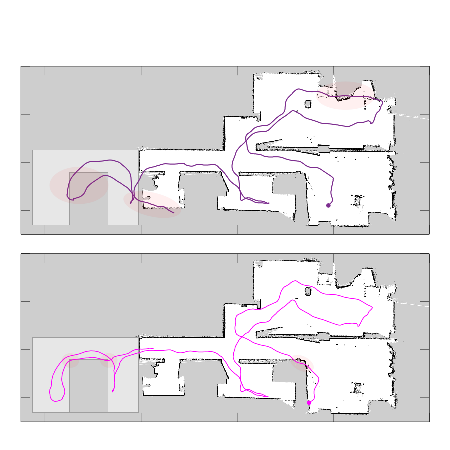
\includegraphics{./figures/11/laser_odometry_fvg_fsm1}}%
    \gplfronttext
  \end{picture}%
\endgroup
